\documentclass{article}
\usepackage[utf8]{inputenc}
\usepackage{cite}
\usepackage{amsthm}
\usepackage{amsmath}
\usepackage{hyperref}
\usepackage{comment}
\usepackage{subfigure}
\usepackage{wrapfig}
\usepackage{float}
\usepackage[colorinlistoftodos]{todonotes}

\begin{document}
\title{Glasses or no glasses classification}
\author{Alesia Sommariva}

\begin{titlepage}
    \begin{center}
        \vspace*{2cm}

        \Large
        \textbf{Glasses or no glasses classification}
        \vspace{0.5cm}
        
        \large
        Statistical methods for machine learning and Algorithms for massive datasets\\ 
        Experimental project report
        \vspace{1.5cm}
        
        Alesia Sommariva\\
        \small
        960824
        \vspace{.5cm}
        
        \normalsize             
        University of Milan\\
        Master's Degree in Computer Science\\
        Academic year 2020/2021
        
        \vfill
        \emph{I declare that this material, which I now submit for assessment, 
        is entirely my own work and has not been taken from the work of others, 
        save and to the extent that such work has been cited and acknowledged within 
        the text of my work. I understand that plagiarism, collusion, and copying 
        are grave and serious offences in the university and accept the penalties that 
        would be imposed should I engage in plagiarism, collusion or copying. 
        This assignment, or any part of it, has not been previously submitted by 
        me or any other person for assessment on this or any other course of study.}

\setlength{\parskip}{0.7em}
    \end{center}
\end{titlepage}


\tableofcontents

\newpage

\section{Introduction}
The project chosen for this report is image classification via convolutional neural network. We address the problem of the classification of images produced by a GAN network containing faces of people who wear / do not wear glasses, both prescription and sunglasses. So, the final objective is to classify wheter the faces in the dataset wear glasses or not.

This project is based on the dataset ``Glasses or no Glasses" published on Kaggle and released under the Attribute-ShareAlike 4.0 Creative Commons license (CC BY-SA 4.0). The neural networks are implemented by using the TensorFlow framework (version 2.6.0), in particular by adopting the Keras library.

We investigate several convolutional neural networks by tuning different parameters in order to find the most simple network with the highest accuracy and lowest loss. It important \\
In section \hyperref[sec:dataset]{2} we present the dataset and the applied preprocessing techniques. In section  \hyperref[sec:cnn]{3} we present the  experiments performed for model selection and discuss the training details. In section \hyperref[sec:cnn]{4} we address the problem of scalability and in section \hyperref[sec:cnn]{5} we present the experiments results and observations.


\section{Dataset overview and preprocessing}
\label{sec:dataset}
In this section we describe the structure of the dataset and the preprocessing techniques applied. The dataset is available at the following link: 
\begin{center}
    \url{https://www.kaggle.com/jeffheaton/glasses-or-no-glasses}
\end{center} 
\subsection{Dataset structure}
The dataset is composed by two \texttt{.csv} files, \texttt{train.csv} and \texttt{test.csv}, conaining the latent vectors and a directory with the pictures generated by those vectors. The \texttt{train.csv} file has 4500 rows and 514 columns: the first one cointains an  unique identifier, the next 512 are latent numbers used by the GAN network and the last one contains the label. The \texttt{test.csv} file has 500 rows and 513 columns: the first one contains the id and the last 512 are the latent numbers. In total there are 5000 images. Each image comes in \texttt{.jpg} file format.

In this project we will use the 4500 labeled images for training, validation and test. The last 500 unlabeled images will be used for final visual testing.
After checking the number of images per class we noticed an imbalance between the two classes, in particular there are more images labeled "glasses" (corresponding to label 1) than "no-glasses" (corresponding to label 0). Indeed there are 1644 images labeled as "glasses" and 2856 labeled as "no-glasses". Moreover, some images did not form clearly, and have the wrong label. This can cause poor performance in training, so it will be taken in consideration.

\subsection{Preprocessing}
We decided to import images in a shape of 100 x 100 x 3 (height, width, colour). Firstly we need to download and decompress the dataset from Kaggle. Then, from the \texttt{train.csv} file we take ids and labels to associate with labeled images, and from \texttt{test.csv} we take the ids to do the same with not labeled images.

RGB channels values are in the [0, 255] range. This range is not ideal for neural network, thus we have to standardize values to be in [0, 1] range.
\\

We found out that $63.47\%$ of the images are labelled as ``glasses", and the other  $36.53\%$ are labeled as ``no glasses`". Therefore, there we have some unbalanced classes. We decided to apply data augmentation by performing some moves, such as random horizontal flip, random rotation of 0.1, and random contrast adjustment of 0.2. Thus, we were able to produce the necessary number of images for the ``no-glasses" class in order to have the same number of images as the ``glasses" class. At the end, we will have 5712 images. 

\begin{figure}[h]
    \centering
    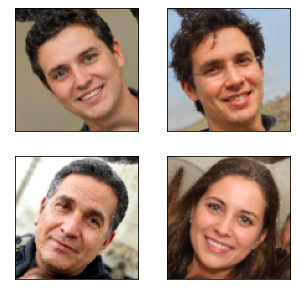
\includegraphics[width=0.2\textwidth]{images/augm_imgs.png}
    \caption{Augmented images}
    \label{fig:augm_imgs}
\end{figure}

In this way we have two datasets: one unbalanced and one balanced over which we will perform model selection (see next section \ref{sec:cnn}).
Following we can see an example of 25 images from the original dataset.

\begin{figure}[H]
    \centering
    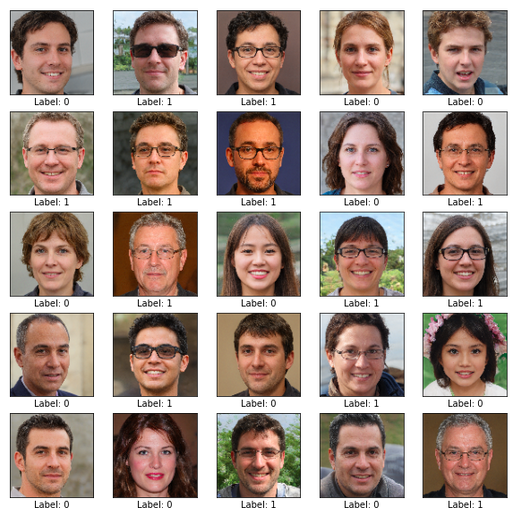
\includegraphics[width=0.5\textwidth]{images/images.png}
    \caption{Images of the original datset}
    \label{fig:train_images}
\end{figure}

\section{CNNs}
\label{sec:cnn}
In this section we describe the experiments performed in order to find the best CNN. We used a  Stratified Cross Validation to tune parameters and also a manual Grid Search for finding out the number of filters in the convolutional layer and the number of blocks (this concept will be described later). We will compare those two approaches.

We decided to do the entire model selection through a ``cascade" mode, along with a grid search, but focused only on two parameters to avoid high computational cost. When we say ``cascade" mode, we mean that for each single parameter we perform a cross validation of 3 fold, for 3 possible values, and then take the values with the best results. We also know, however, that this approach gives a sub-optimal result compared to a complete grid search. However, the complete grid search is computationally much more expensive, and this is why we performed it only on two parameters.

\subsection{Experiments}
Firstly we perform some experiments with different architectures:
\begin{itemize}
    \item First architecture (base): two blocks, each composed by a convolutional layer with ReLu as activation function and a 2D max pooling layer where in the first block we have 16 filters and kernel size of (3,3) in convolutional layer. In the second block we have 32 filters and kernel size of (5,5) with 2 strides. Then a flatten layer, a dense layer of 64 neurons with ReLu as activation function and the last layer with one neuron and sigmoid as activation function. We will use the last layer to get the prediction.
    \item Second architecture (two convolutional layers per block): two blocks composed by two convolutional layers with ReLu as activation function and a 2D max pooling layer. In the first block we have 16 filters and kernel size of (3,3) in convolutional layer, in the second block we have 32 filter and kernel size of (5,5) with 2 strides in convolutional layers. (??? flatten o dense ???) Then a flatten layer, a dense layer of 64 neurons with ReLu as activation function and the last layer with one neuron and sigmoid as activation function.
    \item Third architecture (addition of batch normalization and dropout): in this last architecture we decide to take the previous one and to add a batch normalization layer after each convolutional layer and a dropout of 0.5 between the two final dense layers.
\end{itemize}

All these architectures are trained for 20 epochs, and at the end of each one we tested the model over a validation set in order to observe how the model evolves and performs. In each architecture we have used binary cross entropy as loss function, since we handled a binary classification problem. We used Adam as optimizer to perform the gradient descent. In addition we used a learning rate scheduler callback; this function keeps the learning rate and decreases it exponentially at each epoch. \\

Then, in the case of the unbalanced dataset with the network that obtained the best result depending on the value of the loss,  and in the case of the balanced dataset with the network that obtained the best result depending on the value of the accuracy, we are going to perform tuning over several parameters with Stratified Cross Validation with 3 folds. \\

The parameters and respective values considered for tuning are presented below:
\begin{itemize}
    \item number of blocks: 1, 2, or 3
    \item number of filters on first convolutional layers: 8, 16 and 32 (then doubled and triples on eventual second and third layer)
    \item number of neurons in the fully connected layer: 32, 64 and 128
    \item dropout rate: 0.3, 0.5 and 0.7
\end{itemize}

Cross-validation or KFold Cross Validation systematically creates and evaluates multiple models on multiple subsets of the dataset. This, in turn, provides a population of performance measures. Then we can calculate the mean of these measures to get an idea of how well the procedure performs on average.

With the Cross-validation technique the entire dataset is partitioned in K subsets (also known as folds), in this case K=3, of size $m/K$ each (assume for simplicity that K divides m), where $m$ is the size of the dataset. Basically at each iteration the model is trained on two folds and then tested on the last one. This process runs until each fold has been the test set exactly once.
Then we can calculate the mean of these measures to get an idea of how well the procedure performs on average.

So Stratified Cross Validation extends K-fold Cross Validation by ensuring an equal distribution of the target classes over the splits. This ensures that the classification problem is balanced.
For each fold we then compute the accuracy and loss average, taking in consideration the loss for the unbalanced dataset and the accuracy for the balanced dataset. We will look at the computational cost when the difference of the results is minimal.

For the number of blocks and numbers of filters on convolutional layers we perform also a manual grid search. With this grid search we combine all the possible configurations about the number of blocks and number of filters, performing a cross validation at each iteration. Then we will take the configuration with the best result and compare it with the result obtained from the cascade mode.

\subsubsection{Unbalanced dataset}
After having tested the three starting architectures, the best one turns out to be the last architecture with batch normalization and dropout.

\begin{figure}[h]
    \centering
    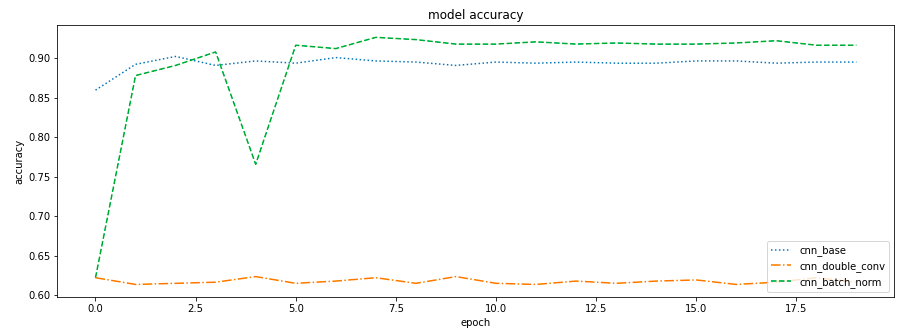
\includegraphics[width=0.7\textwidth]{images/accuracy_unbalance.png}
    \caption{Accuracy}
    \label{fig:acc_unbalance}
\end{figure}

\begin{figure}[h]
    \centering
    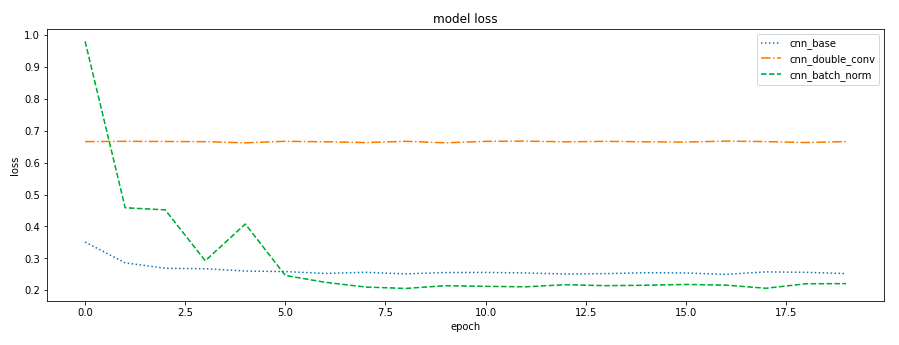
\includegraphics[width=0.7\textwidth]{images/loss_unbalance.png}
    \caption{Loss}
    \label{fig:loss_unbalance}
\end{figure}

Then we performed the model selection with the cascade mode and grid search mode varying the number of blocks and number of filters. 

After this process we chose the architecture resulting from the cascade mode with one single block and 16 filters in the first convolutional layer. The other architecture with 32 filters only perform slightly better and is not worth the additional computational cost.

Continuing the model selection with the cascade mode on the number of neurons and the dropout, the architecture of the final network will have one single block, 16 filters on convolutional layer, 32 neurons on dense layer and a dropout of 0.7, getting an accuracy of $~89.5\%$ and a loss of $~26.1\%$

\subsubsection{Evaluation}
At the end of the model selection we trained the best final model on the train/validation splits of the dataset.
In figure \ref{fig:acc_loss_unb} we can observe the resulting training and loss.

\begin{figure}[h]
    \centering
    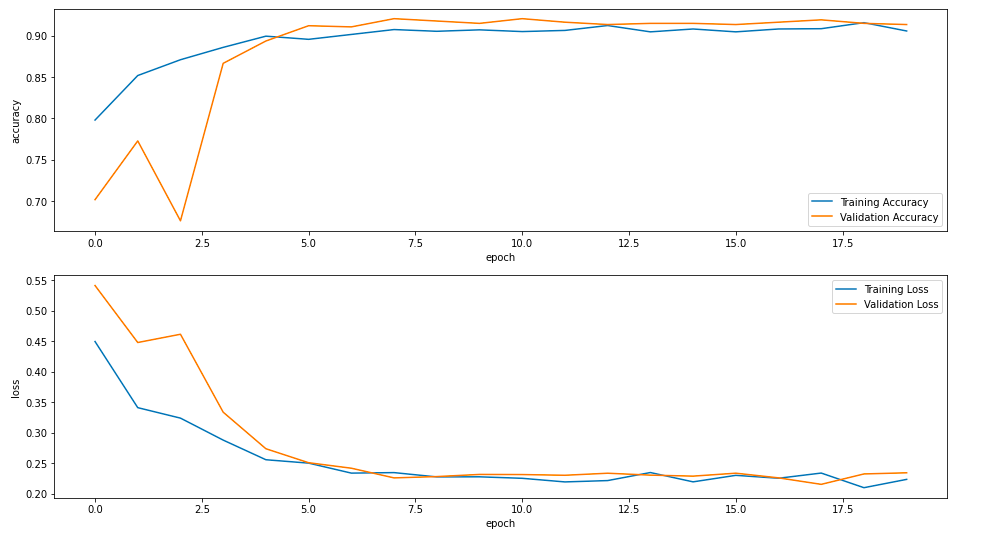
\includegraphics[width=0.8\textwidth]{images/validation_unbalance.png}
    \caption{Accuracy and Loss}
    \label{fig:acc_loss_unb}
\end{figure}

It is interesting to see how already after the tenth epoch validation training and loss attest on extremely similar values and keep them until the end of the epochs, reaching an accuracy of over $0.91$ and a loss of $0.23$, a sign that the neural network is performing well.

Even more remarkable is how well the model generalizes for this train / test split.

\subsubsection{Balanced dataset}
Also in this case the best one turns out to be the third architecture with dropout and batch normalization.

\begin{figure}[H]
    \centering
    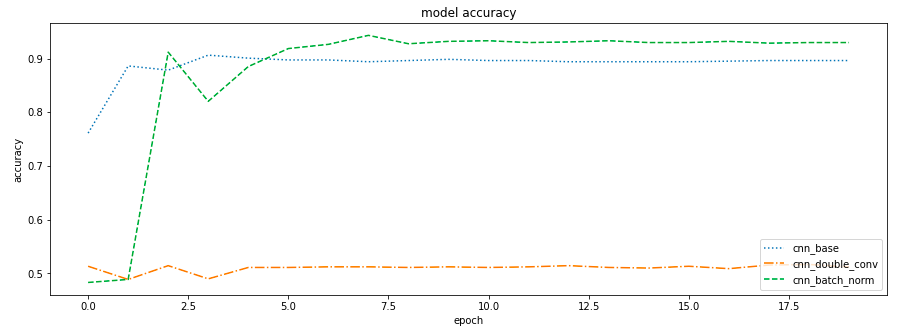
\includegraphics[width=0.7\textwidth]{images/accuracy_balance.png}
    \caption{Accuracy}
    \label{fig:acc_bal}
\end{figure}

\begin{figure}[H]
    \centering
    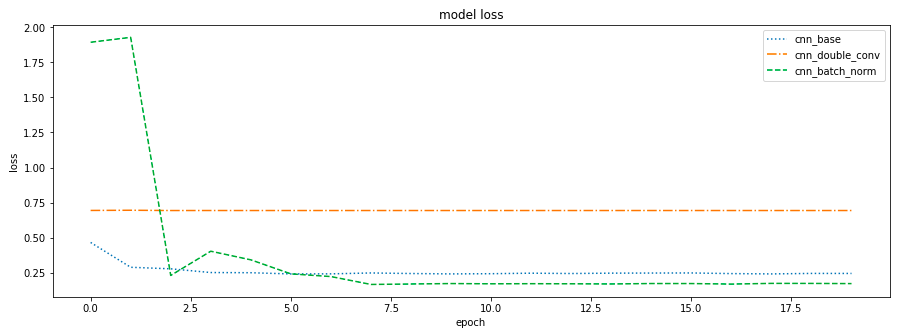
\includegraphics[width=0.7\textwidth]{images/loss_balance.png}
    \caption{Loss}
    \label{fig:loss_bal}
\end{figure}

We executed the same experiments for the unbalanced dataset. So, after first tuning with cascade mode, it appears that 32 filters in the first convolutional layer and one single block is the best architecture. Note that the accuracy in these first experiments already increased to $0.91$ and the loss dropped to $0.20$.\\
After the manually grid search it appears that the best architecture is composed by one single block and 32 filter in the convolutional layer.

So at the end of tuning with the cascade mode for the remaining parameter, i.e. number of neurons in the last but one layer and the dropout, the architecture of the final network will have one single block, 32 filters in the first convolutional layer and 64 neurons with a dropout of 0.7.

\subsubsection{Evaluation}
As before, we  trained  the  best  final  model  on  the train/validation  splits  of  the balanced dataset.

\begin{figure}[H]
    \centering
    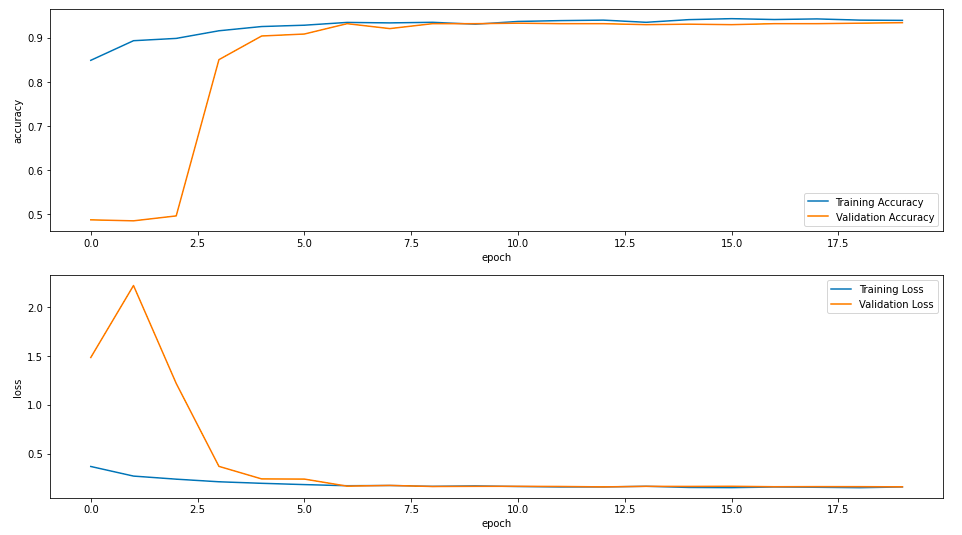
\includegraphics[width=0.8\textwidth]{images/validation_balance.png}
    \caption{Accuracy}
    \label{fig:acc_unbalance}
\end{figure}

It is even more interesting to note how after even fewer epochs than before (about 5), train and loss settle on the same values and keep them until the end, in addition to the fact that the neural network  generalize well and even better than the previous one.
We also have an accuracy of 0.92 and a loss of 0.16



\section{How to scale up with data size}
To cope with this problem first of all we thought of exploiting some methods made available by TensorFlow regarding how to treat the dataset during training: with \texttt{Dataset.cache} we keep the images in memory after having loaded them from the disk during the first epoch. This will ensure that the dataset does not become a bottleneck while training the model. Then, with \texttt{Dataset.shuffle} we perform a complete shuffle at each iteration, in which the size of the shuffle buffer is never less than the size of the set. We use \texttt{Dataset.batch}, which allows us to divide the dataset into batches of 32 samples so that the network takes small amounts of data at a time. Finally we use \texttt{Dataset.prefetch\texttt}, which loads subsequent batches while it is pulling on the current one.

Regarding data storage, we could think of using HDFS, that is a distributed file system that allows you to store data on a cluster of nodes. It allows us to manage large amounts of data that obviously we would never be able to store on a single machine. Thanks to the batch operation on the data we can then load one or more chunks (in a limited number) at a time to form the next batch during the training phase.

\section{Visual Tests}
At the end of the experiments for both the unbalanced and the balanced dataset, we performed a visual test phase over the not labeled images of the dataset. We obtained consistent results with what was seen in the training phase.

\subsection{Test unbalanced dataset}
As we can observe from figure \ref{fig:test_unb}, we have reached a coherent result with nearly $91\%$ accuracy and only one wrong prediction in this case.

\begin{figure}[H]
    \centering
    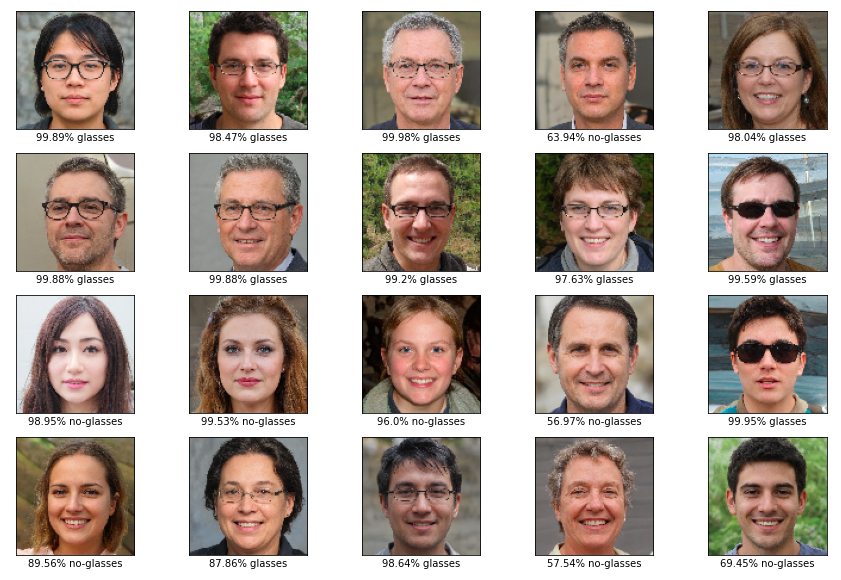
\includegraphics[width=0.7\textwidth]{images/test_unb.png}
    \caption{Visual test over balanced dataset with the respective network}
    \label{fig:test_unb}
\end{figure}

\subsection{Test balanced dataset}
Strangely we cannot say the same thing here (figure \ref{fig:test_bal}), because although we have achieved better results than before we still have two wrong labels.

\begin{figure}[H]
    \centering
    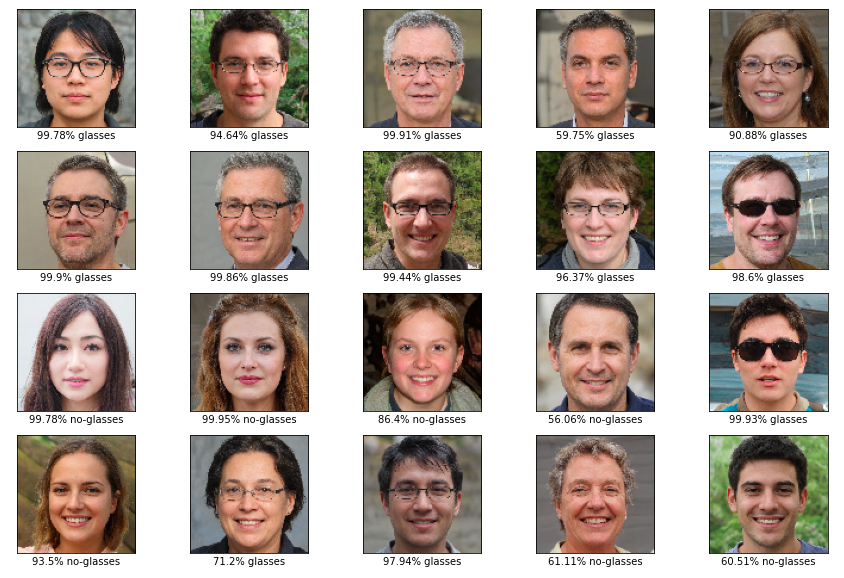
\includegraphics[width=0.7\textwidth]{images/test_bal.png}
    \caption{Visual test over unbalanced dataset with the respective network}
    \label{fig:test_bal}
\end{figure}

\section{Conclusions}
In this project we developed and tested several architectures in order to find the one that gave us the best results. For this purpose, after noticing a slight imbalance in the classes, we decided to create a second dataset by adding images for the class that had the least, via data augmentation. In the first instance, we therefore tested three different architectures. Then with the best performing network we tried to optimize loss and accuracy by tuning some parameters.\\
With the evaluation of the final network in both cases we managed to obtain an improvement, albeit slight.

It is interesting to note that despite the slightly worse performance in the unbalanced dataset, in the visual test we do not even have a prediction error, unlike the case of the balanced dataset where in the same test we have an error.

\end{document}
